% !TEX root = ../../prj4projektdokumentation.tex

\subsection{UART forbindelse til styringsenhed}

Kommunikationen mellem Måleenheden og Styringsenheden er som det fremgår af Figur \ref{fig:Allokering} allokeret på en UART forbindelse. UART kommunikationen foregår via en RX- og en TX-forbindelse mellem enhederne. Opsætning af UART forbindelsen i PSOC creator 4.0 sker ved et blokkald. 

Af Figur \ref{fig:MEUART}, fremgår det at RX og TX forbindelserne på UART blokken er forbundet til to hardware pins på PSOC, henholdsvis Rx\_1 og Tx\_1. Derudover der der forbundet en interrupt-rutine til rx\_interrupt benet. Det er denne forbindelse der sikrer at Måleenheden ender i interrupt-rutinen, som er vist i Figur \ref{fig:MEflowchart}
\begin{figure}[H] % (alternativt [H])
	\centering
	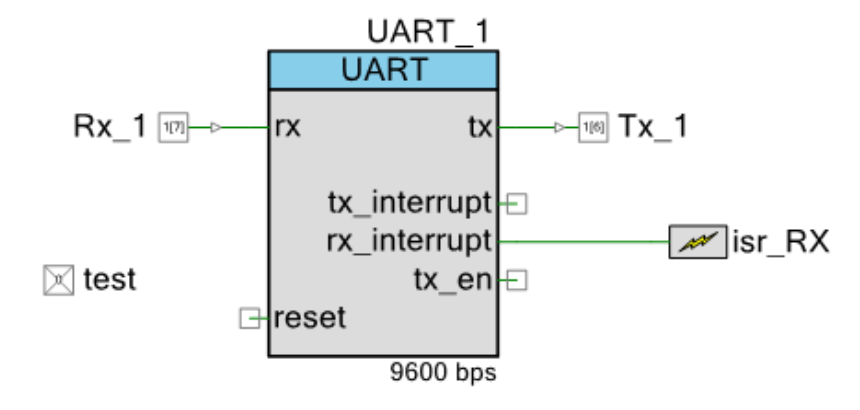
\includegraphics[width=0.5\textwidth]{Figure/MEUART}
	\caption{UART blok fra PSOC creator 4.0}
	\label{fig:MEUART}
\end{figure}

Opsætning af UART fobindelsen er foretaget i henhold til protokollen beskrevet i Kapitel \ref{sec:UARTprotokol}